Game theory is about strategically interdependent decision-making. In such situations the result of a decision also depends on the decisions of others. When making a decision people have to think about what others will do, who in turn are thinking about what others do and so on. Game theory offers several concepts and insights for understanding and analysing such situations and for making better strategic decisions

\begin{definition}[Game Theory]
      Game Theory studies mathematical models of strategic interaction (actions) among rational decision-makers (players).
\end{definition}


\begin{definition}[Normative Game Theory]
      Normative Game Theory is about improving real-world results of games.
\end{definition}


\begin{definition}[Postive Game Theory]
      Positive Game Theory is describing how people behave in real-world situations.
\end{definition}


\begin{definition}[(Non-)cooperative Game Theory]
      A game is cooperative if the players can form binding commitments externally enforced. Cooperative game theory focuses on predicting which coalitions will form, the actions that groups take and the resulting payoffs.

      Non-cooperative game theory , also know as competitive game theory, studies games with competition between individual players.
\end{definition}

\begin{definition}[Action]
      A set $A$ consisting of all the actions $a$ that, under some circumstances, are available to the decision-maker.
\end{definition}


\begin{definition}[Rational choice]
      An action chosen by a decision-maker is at least as good, according to her preferences, like every other available action.
\end{definition}


\begin{note}
      \normalfont  Within game Theory, we assume people can rank any two actions. However, this is not always the case. We are not always 100\% rational.
\end{note}

\begin{definition}[Payoff function]
      The payoff function $u : A \to \rr$ represents a decision-maker’s preferences if, for
      any actions $a, b \in A$
      $$u(a) > u(b) \iff \text{ the decision-maker prefers a to b}$$
\end{definition}

\begin{definition}[Strategic game]
      A strategic game - or normal form game - consists of three things:
      \begin{itemize}[nosep]
            \item a set of players $N$,
            \item for each player a set of actions $A$,
            \item for each player, (ordinal) preferences over the set of action profiles $u_i : A \to \rr$ for all $i \in N$.
      \end{itemize}
\end{definition}


\begin{example}[Prisoner's Dilemma]
      This game has two players. Each player has two actions: Fink or Quiet. The prisoners' dilemma has the action profiles with corresponding payoff:
      \begin{itemize}
            \item If Player 1 and Player 2 each betray the other, each of them serves two years in prison.
            \item If Player 1 betrays Player 2 but Player 2 remains silent, Player 1 will be set free and Player 2 will serve three years in prison (and vice versa)
            \item If Player 1 and Player 2 both remain silent, both of them will serve only one year in prison.
      \end{itemize}
      This can be visualized in the following payoff matrix:
      \begin{table}[h!]
            \begin{center}
                  \begin{tabular}{ c | c c }
                              & Quiet & Fink   \\ \hline
                        Quiet & $2,2$ & $0,3$  \\
                        Fink  & $3,0$ & $1, 1$
                  \end{tabular}
                  \vspace{-5pt}
                  \caption{Payoff matrix corresponding to the Prisoner's Dilemma.}
                  \vspace{-30pt}
            \end{center}
      \end{table}
\end{example}
\begin{theorem}
      Any function applied to the utility which does not change the oridinality\footnote{if $x > y$, then $f(x) > f(y)$}, will not change the game.
\end{theorem}


\begin{example}[Battle of the sexes]
      This game has two players: a wife and a husband. Each player has two actions: Bach or Stravinsky.
      The husband would prefer to go to Bach. The wife would rather go to Stravinsky. Both would prefer to go to the same place rather than different ones.
      This can be visualized in the following payoff matrix:
      \begin{table}[h!]
            \begin{center}
                  \begin{tabular}{ c | c c }
                                   & Bach  & Stravinsky \\ \hline
                        Bach       & $2,1$ & $0,0$      \\
                        Stravinsky & $0,0$ & $1, 2$
                  \end{tabular}
                  \vspace{-5pt}
                  \caption{Payoff matrix corresponding to the Battle of the sexes.}
                  \vspace{-30pt}
            \end{center}
      \end{table}
\end{example}


\begin{example}[Stag hunt]
      This game has two players: two identical hunters. Each hunter can individually choose to hunt a stag or hunt a hare. If an individual hunts a stag, they must have the cooperation of their partner to succeed. An individual can get a hare by himself, but a hare is worth less than a stag.
      This can be visualized in the following payoff matrix:
      \begin{table}[h!]
            \begin{center}
                  \begin{tabular}{ c | c c }
                             & Stag  & Hare   \\ \hline
                        Stag & $2,2$ & $0,1$  \\
                        Hare & $1,0$ & $1, 1$
                  \end{tabular}
                  \vspace{-10pt}
                  \caption{Payoff matrix corresponding to Stag Hunt.}
                  \vspace{-20pt}
            \end{center}
      \end{table}
\end{example}


\begin{definition}[Nash equilibrium]
      A Nash equilibrium is an action profile with the property that no player can do better given that other players adhere to their actions.
      \textit{Formally:} the action profile $a^*$ in a strategic game with ordinal preferences is a Nash
      equilibrium if, for every player $i$ and every action $a_i$ of player $i$, $a^*$ is at least as good
      according to player $i$'s preferences as the action profile $(a_i , a^*_{-i})$ in which $i$ chooses $a_i$
      while every other player $j$ chooses $a^*_j$.

      Or, for every player $i$
      \[
            u_i (a^*) > u_i(a_i , a^*_{-i} )
      \]
      for every action $a_i$ of player $i$ where $u_i$ represents player $i$'s preferences.
\end{definition}

\begin{definition}[Best Response]
      The Best Response for player $i$ is the set of player $i$'s best actions (denoted by $\mathcal{B}_i (a_{-i})$) when the list of the other
      players' actions is $a_{-i}$
      \textit{Formally}:
      \[
            \mathcal{B}_i (a_{-i}) = \{a_i \mid a_i \in A_i : u_i (a_i ,a_{-i} ) > u_i (a_i' ,a_{-i} )  \forall a_i' \in A_i\}
      \]
\end{definition}
\begin{corollary}
      In a Nash equilibrium every player plays best response to the other players' actions. \textit{Formally:}
      \[
            a^* \text{ is Nash equilibrium} \iff a^*_i \in \mathcal{B}_i (a^*_{-i} ) \forall i
      \]
\end{corollary}


\begin{definition}[Strictly dominating actions]
      We say a player $i$'s action $a_i''$ strictly dominates action $a_i'$ if
      \[u_i (a_i'' , a_{-i} ) > u_i (a_i' , a_{-i} )\]
      for every list of other players' actions $a_{-i}$. 
      
      This means that a player’s action strictly dominates another action if it 
      is superior, no matter what the other players do.
\end{definition}


\begin{definition}[Strictly dominated actions]
      If an action strictly dominates the action $a_i$, we say that $a_i$ is strictly dominated.
\end{definition}


\begin{corollary}
      \normalfont A strictly dominated action is not used in any Nash equilibrium.
\end{corollary}


\begin{definition}[Weakly Dominated actions]
      We say a player $i$'s action $a_i''$ strictly dominates action $a_i'$ if
      \[
            u_i (a_i'' , a_{-i} ) \ge u_i (a_i' , a_{-i} )
      \]
      for every list of other players' actions $a_{-i}$, and
      \[
            u_i (a_i'' , a_{-i} ) > u_i (a_i' , a_{-i} )
      \]
      for some list $a_{-i}$ of other players' actions.
\end{definition}


\begin{note}
      \normalfont A Weakly dominated action may be used in a Nash equilibrium.
\end{note}


\begin{example}
      Consider the following payoff matrix:
      \begin{table}[h!]
            \begin{center}
                  \begin{tabular}{ c | c c }
                              & Left  & Right  \\ \hline
                        Left  & $2,2$ & $0,3$  \\
                        Right & $3,0$ & $1, 1$
                  \end{tabular}
                  \caption{Payoff matrix corresponding to the Prisoner's Dilemma.}
            \end{center}
      \end{table}
      \vspace{-15pt}

      Row Player's action \textit{Bottom} is weakly dominated by \textit{Top}
      Column Player's action \textit{Right} is weakly dominated by \textit{Left}
      Nevertheless, there are two Nash equilibria: (\textit{Top}, \textit{Left}) and (\textit{Bottom}, \textit{Right}).
\end{example}


\begin{illustration}[Contributing to a public good]
      When building some public good (like street lights), there is a cost to that ($c_i$) and a value function ($v_i(c)$). Furthermore, each player has a maximum ($w_i$) they can contribute. This gives the following game:
      \begin{itemize}
            \item Players: two people.
            \item Actions: $0 < c_i < w_i$ .
            \item Preferences: $u_i (c_1 , c_2 ) = v_i (c_1 +c_2 ) - c_i$ for $i=1,2$.
      \end{itemize}

      Consider the perspective of player 1. 
      We assume $0 < \mathcal{B}_1(0) < w_1$ where $\mathcal{B}_1(0)$ is the best response when the other player contributes $0$.   
      Suppose that $u_1 (c_1 ,0)$ has an interior maximum thus $b_1(0)$ is player 1's best response to $c_ 2 = 0$;
      Now consider $\mathcal{B}_1(k)$, 1's best response to $c_2 = k$:
      \begin{align*}
            u_1(c_1 +k,0) & = v_1 (c_1 +k) - c_1 - k; \\
            u_1(c_1 ,k)   & = v_1 (c_1 +k) - c_1 ;
      \end{align*}
      Now it follows, by adding $k$ to both sides:
      \begin{align*}
            u_1(c_1 +k,0) + k & = v_1 (c_1 +k) - c_1 ; \\
            u_1(c_1 ,k)       & = v_1 (c_1 +k) - c_1 ;
      \end{align*}
      Therefore,
      \[
            u_1(c_1 ,k) =u_1(c_1 +k,0) + k;
      \]
      This means: for me to be indifferent to spend $c_1$ euros and player 2 spending $k$ euros or spending $c_1$ euros, player 2 spending $0$ and receiving $k$ euros.

      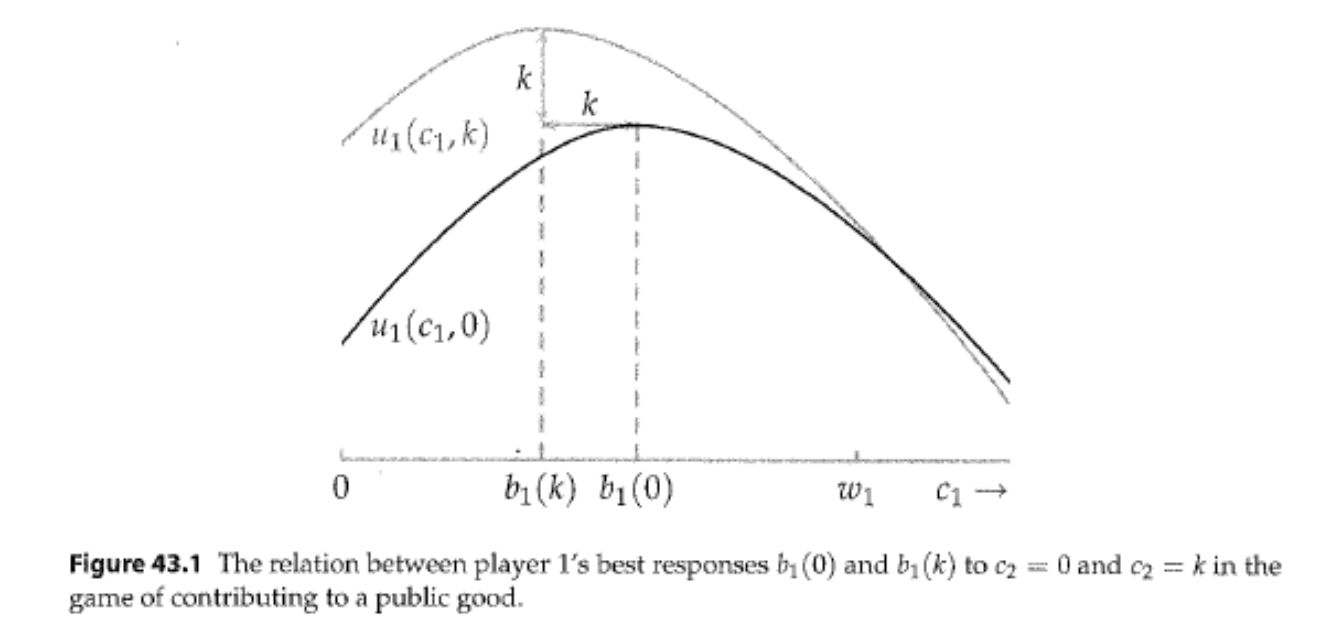
\includegraphics[width=1\textwidth]{im1.png}

      We now can say:
      if $k<b_1 (0)$ then $b_1(k)=b_1(0)- k$;
      if $k>b_1 (0)$ then $b_1( k)=0$;
      When doing a similar analysis applies to player 2: assume $b_1 (0) > b_2(0)$. Now we can say:
      if $k<b_2 (0)$ then $b_2(k)=b_2(0)- k$;
      if $k>b_2 (0)$ then $b_2(k)=0$;

      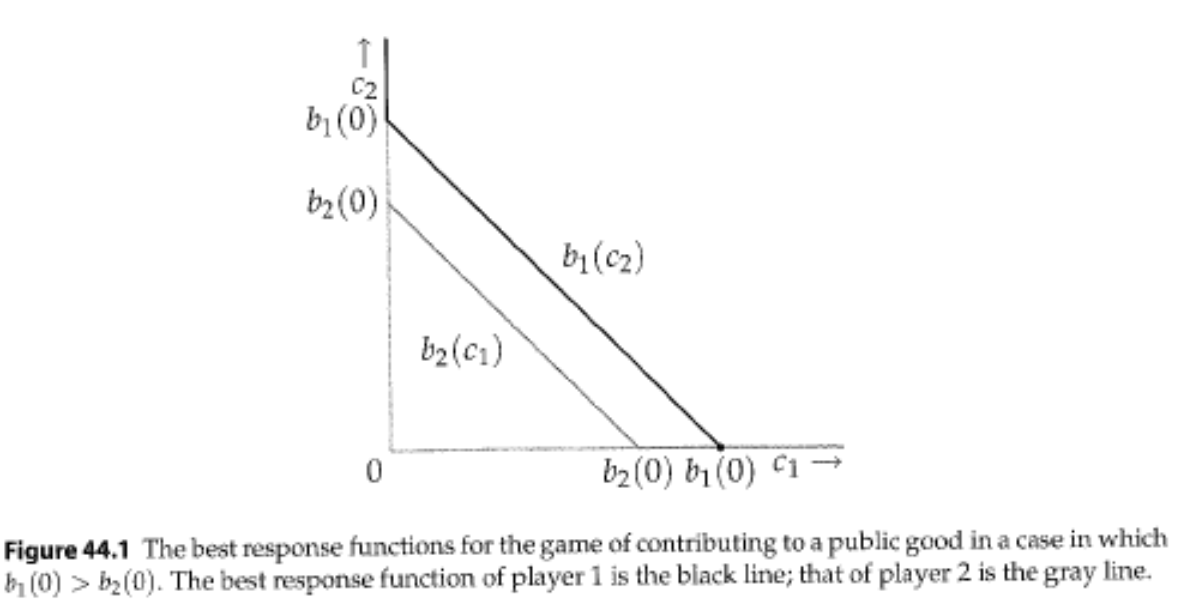
\includegraphics[width=1\textwidth]{im2.png}

      Since each player chooses best response, from the Graph it follows: $(b_1(0),0)$ is the Nash equilibrium if $b_1(0) > b_2(0)$. When $b_1(0) = b_2(0)$, the Nash equilibrium are all $(c_1,c_2) : c_1+c_2 = b_1(0) = b_2(0), c_1, c_2 \ge 0$. Lastly, when $b_1(0) < b_2(0)$,the Nash equilibrium is $(0,b_2(0))$.
\end{illustration}


\begin{definition}[Symmetric games]
      A strategic game with ordinal preferences is a \textbf{symmetric game} if the players' sets
      of actions are the same and the players' preferences are represented by $u_i$ with
      $u_i(a i , a_{-i} ) = u_j (a_j , a_{-j} )$ for all $i,j$.
\end{definition}


\begin{definition}[Symmetric Nash equilibrium]
      An action profile $a^*$ in a symmetric game is a \textbf{symmetric Nash equilibrium} if it is a Nash equilibrium and $a^*_i$ is the same for each player $i$.
\end{definition}